% ═══════════════════════════════════════════════════════════════════════════════
% The Quantum Millionaire Mind
% Secrets of Blockchain Wealth from the Q-NarwhalKnight Founder
% ═══════════════════════════════════════════════════════════════════════════════
\documentclass[11pt,a4paper]{article}

% ── Encoding & Fonts ──────────────────────────────────────────────────────────
\usepackage[utf8]{inputenc}
\usepackage[T1]{fontenc}
\usepackage{lmodern}

% ── Page Geometry ─────────────────────────────────────────────────────────────
\usepackage{geometry}
\geometry{margin=1in}

% ── Core Packages ─────────────────────────────────────────────────────────────
\usepackage{amsmath,amssymb}
\usepackage{graphicx}
\usepackage{booktabs}
\usepackage{enumitem}
\usepackage{float}
\usepackage{caption}
\usepackage{titlesec}
\usepackage{fancyhdr}
\usepackage{xcolor}
\usepackage{hyperref}
\usepackage{tikz}
\usepackage[most]{tcolorbox}
\usepackage{listings}
\usepackage{epigraph}
\usepackage{csquotes}
\usepackage{setspace}
\usepackage{parskip}

% ── TikZ Libraries ───────────────────────────────────────────────────────────
\usetikzlibrary{arrows.meta,positioning,shapes.geometric,calc,decorations.pathmorphing,patterns}

% ── Colors ────────────────────────────────────────────────────────────────────
\definecolor{qnkblue}{RGB}{30,90,150}
\definecolor{qnkgold}{RGB}{180,140,40}
\definecolor{qugblue}{HTML}{3B82F6}
\definecolor{quggold}{HTML}{F59E0B}
\definecolor{quggreen}{HTML}{10B981}
\definecolor{qugpurple}{HTML}{8B5CF6}
\definecolor{codebg}{RGB}{245,245,245}
\definecolor{darkrust}{RGB}{120,40,20}
\definecolor{ekerred}{RGB}{180,40,40}
\definecolor{wealthgold}{RGB}{212,175,55}

% ── Hyperref Setup ────────────────────────────────────────────────────────────
\hypersetup{
    pdftitle={The Quantum Millionaire Mind},
    pdfauthor={Q-NarwhalKnight Development Team},
    colorlinks=true,
    linkcolor=qnkblue,
    citecolor=qnkblue,
    urlcolor=qugpurple,
}

% ── Section Formatting ────────────────────────────────────────────────────────
\titleformat{\section}{\Large\bfseries\color{qnkblue}}{\thesection}{1em}{}
\titleformat{\subsection}{\large\bfseries\color{qnkblue!80}}{\thesubsection}{1em}{}
\titleformat{\subsubsection}{\normalsize\bfseries\color{qnkblue!60}}{\thesubsubsection}{1em}{}

% ── Header/Footer ─────────────────────────────────────────────────────────────
\pagestyle{fancy}
\fancyhf{}
\fancyhead[L]{\small\color{gray}The Quantum Millionaire Mind}
\fancyhead[R]{\small\color{gray}\thepage}
\fancyfoot[C]{\small\color{gray!60}Q-NarwhalKnight --- \url{https://quillon.xyz}}
\renewcommand{\headrulewidth}{0.4pt}

% ── Code Listings ─────────────────────────────────────────────────────────────
\lstdefinelanguage{Rust}{
    morekeywords={fn, let, mut, pub, struct, impl, self, if, else, for, while,
                  loop, match, return, use, mod, crate, super, where, trait,
                  type, as, in, const, static, ref, move, async, await, true,
                  false, u64, u128, f64, Vec, String, Result, Ok, Err, Some, None},
    morecomment=[l]{//},
    morecomment=[s]{/*}{*/},
    morestring=[b]",
    sensitive=true,
}

\lstset{
    language=Rust,
    backgroundcolor=\color{codebg},
    basicstyle=\ttfamily\footnotesize,
    breaklines=true,
    frame=single,
    rulecolor=\color{gray!30},
    numbers=left,
    numberstyle=\tiny\color{gray},
    numbersep=5pt,
    showspaces=false,
    showstringspaces=false,
    keywordstyle=\color{qugpurple}\bfseries,
    commentstyle=\color{quggreen!70!black}\itshape,
    stringstyle=\color{ekerred},
    tabsize=4,
    xleftmargin=1.5em,
    framexleftmargin=1.5em,
}

% ── Custom Boxes ──────────────────────────────────────────────────────────────
\newtcolorbox{wealthfile}[1][]{
    colback=wealthgold!8,
    colframe=wealthgold!80!black,
    fonttitle=\bfseries\large\color{wealthgold!30!black},
    title={{\small\faIcon{lightbulb}} Wealth File},
    coltitle=wealthgold!30!black,
    boxrule=1.5pt,
    arc=4pt,
    left=10pt,
    right=10pt,
    top=8pt,
    bottom=8pt,
    before upper={\itshape\color{black!80}},
    #1
}

% Simpler version without fontawesome (which may not be installed)
\newtcolorbox{wealthbox}[1][]{
    colback=wealthgold!8,
    colframe=wealthgold!80!black,
    fonttitle=\bfseries\large\color{wealthgold!30!black},
    title={\raisebox{-0.5pt}{\tiny$\bigstar$} Wealth File},
    boxrule=1.5pt,
    arc=4pt,
    left=10pt,
    right=10pt,
    top=8pt,
    bottom=8pt,
    before upper={\itshape\color{black!80}},
    #1
}

\newtcolorbox{codestory}[1][]{
    colback=qnkblue!5,
    colframe=qnkblue!70,
    fonttitle=\bfseries\color{qnkblue!90},
    boxrule=1pt,
    arc=3pt,
    left=8pt,
    right=8pt,
    #1
}

\newtcolorbox{declaration}[1][]{
    colback=qugpurple!5,
    colframe=qugpurple!60,
    fonttitle=\bfseries\color{qugpurple},
    boxrule=1.5pt,
    arc=4pt,
    left=10pt,
    right=10pt,
    top=8pt,
    bottom=8pt,
    #1
}

\newtcolorbox{principle}[1][]{
    colback=quggreen!5,
    colframe=quggreen!60,
    fonttitle=\bfseries\color{quggreen!80!black},
    boxrule=1pt,
    arc=3pt,
    left=8pt,
    right=8pt,
    #1
}

% ── Epigraph Styling ─────────────────────────────────────────────────────────
\setlength{\epigraphwidth}{0.75\textwidth}
\renewcommand{\epigraphflush}{center}
\renewcommand{\epigraphrule}{0pt}

% ═══════════════════════════════════════════════════════════════════════════════
% DOCUMENT
% ═══════════════════════════════════════════════════════════════════════════════
\begin{document}

% ── Title Page ────────────────────────────────────────────────────────────────
\begin{titlepage}
\centering
\vspace*{1.5cm}

% Title decoration

\begin{tikzpicture}
    \draw[wealthgold, line width=2pt] (-5,0) -- (5,0);
    \node[wealthgold, font=\Large] at (0,0.4) {$\bigstar$};
\end{tikzpicture}

\vspace{0.8cm}

{\Huge\bfseries\color{qnkblue} The Quantum\\[0.3cm]
Millionaire Mind\\[0.5cm]}

{\LARGE\color{wealthgold!80!black}\itshape
Secrets of Blockchain Wealth\\
from the Q-NarwhalKnight Founder\\[0.8cm]}


\begin{tikzpicture}
    \draw[wealthgold, line width=1pt] (-4,0) -- (4,0);
\end{tikzpicture}

\vspace{0.6cm}

{\large\color{gray}
Inspired by T. Harv Eker's \emph{Secrets of the Millionaire Mind}\\[0.3cm]
Applied to building a quantum-resistant blockchain from zero to mainnet\\[1cm]}

% Abstract box
\begin{tcolorbox}[
    colback=qnkblue!5,
    colframe=qnkblue!60,
    width=0.85\textwidth,
    arc=6pt,
    boxrule=1pt,
    left=12pt,
    right=12pt,
    top=10pt,
    bottom=10pt,
]
\small
\textbf{Abstract.}
Every person carries a financial blueprint---a set of beliefs and habits
etched in the subconscious that determines their financial destiny.
T.~Harv Eker taught that to change your financial life, you must first
rewrite your money blueprint. This paper tells the story of a founder
who did exactly that---not in a journal, but in Rust. Eighty-plus
crates. A 21-million-coin emission schedule spanning 256~years.
Post-quantum cryptography for threats decades away. And a transparent
1.9\% founder fee encoded immutably in consensus, so that every
gigahash of mining power becomes passive income---not a salary,
but a financial blueprint made permanent in code.

Where Eker rewired his thermostat with affirmations, this founder
rewired his with \texttt{u128} arithmetic and 4{,}000 tests.
\end{tcolorbox}

\vspace{1cm}

{\large\bfseries Q-NarwhalKnight Whitepaper\\[0.3cm]}
{\large February 2026\\[0.5cm]}
{\color{gray}\small Version 1.0}

\vfill


\begin{tikzpicture}
    \draw[wealthgold, line width=1pt] (-5,0) -- (5,0);
\end{tikzpicture}

\vspace{0.3cm}

{\small\color{gray}
Q-NarwhalKnight Development Team\\
\url{https://quillon.xyz}
}
\end{titlepage}

% ── Table of Contents ─────────────────────────────────────────────────────────
\newpage
\tableofcontents
\newpage

% ═══════════════════════════════════════════════════════════════════════════════
% PART I: THE BLUEPRINT
% ═══════════════════════════════════════════════════════════════════════════════

\begin{center}
{\LARGE\bfseries\color{qnkblue} Part I: The Blueprint}\\[0.3cm]

\begin{tikzpicture}
    \draw[qnkblue, line width=1pt] (-3,0) -- (3,0);
\end{tikzpicture}
\end{center}
\vspace{0.5cm}

% ── Chapter 1 ─────────────────────────────────────────────────────────────────
\section{Your Code Is Your Financial Blueprint}

\epigraph{``Your income can grow only to the extent that you do.''}%
{---T. Harv Eker, \emph{Secrets of the Millionaire Mind}}

\begin{wealthbox}[title={\raisebox{-0.5pt}{\tiny$\bigstar$} Wealth File \#1}]
``Your money blueprint determines your financial life. If your blueprint
is set for earning \$50,000 a year, that's exactly what you'll make---not
a penny more. To change your financial life, you must first change your
financial blueprint.''
\end{wealthbox}

\vspace{0.3cm}

Most people's financial blueprints live in their subconscious---inherited
from parents, shaped by childhood, reinforced by society. They are invisible
and, precisely because of that, almost impossible to change.

But what if you could write your financial blueprint in a language so
precise that it compiles to machine code? What if your relationship with
money were not a vague feeling but a set of constants, checked by a
compiler, verified by 4{,}000 tests, and enforced by cryptographic
consensus across every node on the planet?

That is exactly what the founder of Q-NarwhalKnight did.

The blueprint began with three lines of Rust:

\begin{lstlisting}[caption={The Financial Blueprint in Code (\texttt{emission\_controller.rs})}]
/// Maximum supply: 21,000,000 QUG with 24 decimal places
pub const QUG_MAX_SUPPLY: u128 =
    21_000_000_000_000_000_000_000_000_000_000;

/// Base annual emission for Era 0: 2,625,000 QUG
pub const BASE_ANNUAL_EMISSION: u128 =
    2_625_000_000_000_000_000_000_000_000_000;

/// Seconds per halving era: 4 years (Julian)
pub const SECONDS_PER_HALVING: u64 = 126_230_400;
\end{lstlisting}

Twenty-one million coins. Four-year halving cycles. A 256-year emission
schedule computed with \texttt{u128} fixed-point arithmetic at $10^{24}$
decimal precision. No floating-point rounding errors. No ambiguity. No
``I think I deserve more.'' The entire monetary universe of QUG is
defined by three constants and the math that flows from them.

Eker says your blueprint is your thermostat---set it to 72~degrees and
the system will always return to 72, no matter how hot or cold it gets
outside. In Q-NarwhalKnight, the thermostat is the
\texttt{EmissionController}: a feedback loop that measures real block
rates, computes the ideal reward, applies an error-correction factor,
and ensures the network converges on exactly 2{,}625{,}000~QUG per year
in Era~0---no more, no less.

Most thermostats are invisible. This one is open-source.

\begin{principle}[title={\textbf{The Principle}}]
Most people inherit a financial blueprint they never examine.
The founder's first act was to write one from scratch---in a language
that refuses to compile ambiguity.
\end{principle}

% ── Chapter 2 ─────────────────────────────────────────────────────────────────
\section{Rich People Think Big, Poor People Think Small}

\epigraph{``If you shoot for the stars, you'll at least hit the moon.''}%
{---T. Harv Eker}

\begin{wealthbox}[title={\raisebox{-0.5pt}{\tiny$\bigstar$} Wealth File \#2}]
``Big thinking and big actions lead to having both money and meaning.
The size of the problem is never the issue---what matters is the size
of you.''
\end{wealthbox}

\vspace{0.3cm}

When the founder started writing Q-NarwhalKnight, the sensible advice was:
``Just fork Bitcoin.'' Or: ``Use Substrate.'' Or: ``Nobody needs another
blockchain---and certainly not one with quantum cryptography for threats
that won't exist for twenty years.''

The founder thought big anyway. Sensible advice, after all, is the
financial blueprint of the middle class:

\begin{itemize}[leftmargin=2em]
    \item \textbf{80+ Rust crates} across consensus, networking, storage,
          mining, privacy, DEX, smart contracts, AI inference, TUI, GUI,
          Tor integration, and bounty systems.
    \item \textbf{Post-quantum cryptography}---Dilithium5, Kyber1024,
          SPHINCS+---for threats decades away, because ``the best time to
          prepare for a quantum computer is before one exists.''
    \item \textbf{A 256-year emission schedule} spanning 64 halving eras,
          with mathematical precision that accounts for leap years using
          the Julian-year convention ($365.25 \times 86{,}400 =
          31{,}557{,}600$~seconds).
    \item \textbf{Tor privacy circuits}---four dedicated circuits per
          validator, rotated every epoch, with a Dandelion++ gossip
          protocol for traffic-analysis resistance.
    \item \textbf{An embedded DEX} with AMM liquidity pools, 24-decimal
          precision arithmetic, and overflow-safe \texttt{u128} math.
    \item \textbf{Smart contracts} via a WASM virtual machine with
          gas metering and a collateral-vault system.
\end{itemize}

Every one of these was built from scratch---not forked, not copied, not
``inspired by.'' Eighty crates, each with its own \texttt{Cargo.toml},
its own test suite, its own reason for existing.

Eker would recognize this instantly: it is the difference between a
``small-thinking'' fork that copies someone else's blueprint and a
``big-thinking'' architecture that dares to define its own.

The workspace \texttt{Cargo.toml} tells the story:

\begin{lstlisting}[caption={The Scale of Ambition (\texttt{Cargo.toml}, abbreviated)}]
[workspace]
members = [
    "crates/q-api-server",     # REST API + block producer
    "crates/q-storage",        # RocksDB engine + emission
    "crates/q-network",        # libp2p gossipsub + DHT
    "crates/q-types",          # Consensus types + crypto
    "crates/q-mining",         # Mining engine + dev fee
    "crates/q-dex",            # AMM DEX with LP pools
    "crates/q-tor-client",     # Embedded Tor (arti)
    "crates/q-tor-circuit",    # Dedicated circuit mgmt
    "crates/q-vm",             # WASM smart contracts
    "crates/q-stablecoin",     # Algorithmic stablecoin
    "crates/q-dandelion",      # Dandelion++ privacy
    "crates/q-bounty-protocol",# Bug bounty system
    # ... 70+ more crates
]
\end{lstlisting}

\begin{principle}[title={\textbf{The Principle}}]
Small thinkers fork. Big thinkers build from first principles.
The size of your codebase reflects the size of your vision.
\end{principle}


% ── Chapter 3 ─────────────────────────────────────────────────────────────────
\section{Rich People Are Committed, Poor People Want to Be Rich}

\epigraph{``The number one reason most people don't get what they want
is that they don't know what they want. Rich people are totally clear
that they want wealth.''}%
{---T. Harv Eker}

\begin{wealthbox}[title={\raisebox{-0.5pt}{\tiny$\bigstar$} Wealth File \#3}]
``There is a difference between being interested in something and being
committed to it. When you're interested, you do what's convenient.
When you're committed, you accept no excuses---only results.''
\end{wealthbox}

\vspace{0.3cm}

Commitment is not glamorous. Commitment is a 3~AM debug session when
the emission controller has a 34$\times$ overshoot because someone
added three extra zeros to \texttt{BASE\_ANNUAL\_EMISSION}:

\begin{codestory}[title={\textbf{The 34$\times$ Emission Overshoot (Feb 9, 2026)}}]
\small
The emission controller was minting 34 times the intended supply.
The constant \texttt{BASE\_ANNUAL\_EMISSION} had $10^{27}$ instead of
$10^{24}$---three zeros too many in a 31-digit number. Meanwhile,
\texttt{add\_block()} was defined but never called, so the block-rate
measurement was wrong too.

The fix required:
\begin{enumerate}[leftmargin=2em]
    \item Correcting the constant (count every zero in a 24-decimal number)
    \item Wiring \texttt{track\_block\_for\_emission()} into
          \texttt{balance\_consensus.rs} for all blocks---local and P2P
    \item Verifying the fix didn't break 4{,}000+ existing tests
\end{enumerate}
\end{codestory}

\vspace{0.3cm}

Commitment is the 26.9~GB memory leak at 2~AM:

\begin{codestory}[title={\textbf{The RocksDB Memory Leak (Feb 19, 2026)}}]
\small
Beta server grew to 26.9~GB RSS and got OOM-killed. RocksDB was
auto-configuring its block cache to one-third of total RAM---16~GB
on the production server. The fix:
\texttt{ROCKSDB\_BLOCK\_CACHE\_MB=4096} in the systemd service file.
Four characters of configuration. Three hours of diagnosis.
That ratio---hours of detective work for a one-line fix---is the hidden
cost of every line of infrastructure code ever written.
\end{codestory}

\vspace{0.3cm}

Commitment is the height regression that nearly wiped the chain:

\begin{codestory}[title={\textbf{The Height Regression (Feb 19, 2026)}}]
\small
Node restarted at height 5{,}431 and came back at 2{,}502. The
fast-recovery threshold was \texttt{> 10\_000}---at height 5{,}431, the
node fell through to a genesis scan that returned 2{,}502. Additionally,
\texttt{save\_safe\_floor()} used a non-synced \texttt{put()} instead of
\texttt{put\_sync()} with \texttt{fsync}. The write looked successful but
never reached disk.

\texttt{cargo clean \&\& cargo build --release}---while the world sleeps.
\end{codestory}

\vspace{0.3cm}

Eker's distinction is precise: wanting to be rich is a fantasy.
Commitment means you fix the bug at 3~AM because 27~miners depend on
your node. You do not complain. You do not take a break. You
\texttt{cargo clean --package q-storage} and rebuild, because
incremental compilation cached the old constant and you cannot trust it.

A wish compiles to nothing. Commitment compiles to a release binary.

\begin{principle}[title={\textbf{The Principle}}]
Wanting to build a blockchain is a wish. Commitment is counting zeros
in a 31-digit constant at 3~AM and not stopping until the tests pass.
\end{principle}


% ═══════════════════════════════════════════════════════════════════════════════
% PART II: THE 1.9% PRINCIPLE
% ═══════════════════════════════════════════════════════════════════════════════
\newpage
\begin{center}
{\LARGE\bfseries\color{wealthgold!80!black} Part II: The 1.9\% Principle}\\[0.3cm]
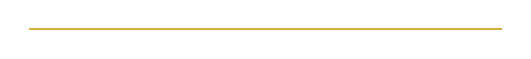
\begin{tikzpicture}
    \draw[wealthgold, line width=1pt] (-3,0) -- (3,0);
\end{tikzpicture}
\end{center}
\vspace{0.5cm}


% ── Chapter 4 ─────────────────────────────────────────────────────────────────
\section{The Wealth File: 1.9 Percent of Everything}

\epigraph{``Rich people focus on their net worth.\\
Poor people focus on their working income.''}%
{---T. Harv Eker}

\begin{wealthbox}[title={\raisebox{-0.5pt}{\tiny$\bigstar$} Wealth File \#4}]
``The true measure of wealth is net worth, not working income.
Working income is important, but it is only one of four factors in
your net worth---and not the most important one. Net worth includes
income, savings, investments, and simplification.''
\end{wealthbox}

\vspace{0.3cm}

The founder could have paid themselves a salary. A monthly wire transfer.
An hourly rate. That is what employees do---trade time for money, the
financial blueprint of the working class.

Instead, the founder wrote seven lines of Rust:

\begin{lstlisting}[caption={The 1.9\% Fee in Consensus (\texttt{block\_producer.rs})}]
// v7.1.5: Configurable dev fee (basis points)
let dev_fee_bps_val = self.dev_fee_bps
    .load(std::sync::atomic::Ordering::Relaxed) as u128;
const BPS_DIVISOR: u128 = 10_000;
const FOUNDER_WALLET_HEX: &str =
    "efca1e8c1f46e91013b4073898c771bb3d566453537ccf87\
     e834505925e50723";

// Integer-only fee calculation for cross-platform determinism
let dev_fee_amount = total_reward
    .saturating_mul(dev_fee_bps_val) / BPS_DIVISOR;
let miner_reward = total_reward
    .saturating_sub(dev_fee_amount);
\end{lstlisting}

Not a salary. A \emph{percentage}. 1.9\% of every block reward, from
every miner, on every node, for as long as the chain lives---or until
the last of the 21{,}000{,}000~QUG is minted, approximately 256~years
from now.

Let the math speak:

\begin{table}[H]
\centering
\caption{The 1.9\% Fee Across the Emission Schedule}
\begin{tabular}{@{}lrrr@{}}
\toprule
\textbf{Era} & \textbf{Annual Emission (QUG)} & \textbf{1.9\% (QUG/yr)} & \textbf{Miners (QUG/yr)} \\
\midrule
0 (Years 1--4)   & 2{,}625{,}000 & 49{,}875  & 2{,}575{,}125 \\
1 (Years 5--8)   & 1{,}312{,}500 & 24{,}937  & 1{,}287{,}563 \\
2 (Years 9--12)  &   656{,}250   & 12{,}469  &   643{,}781   \\
3 (Years 13--16) &   328{,}125   &  6{,}234  &   321{,}891   \\
\midrule
\textbf{Lifetime (64 eras)} & \textbf{21{,}000{,}000} & \textbf{399{,}000} & \textbf{20{,}601{,}000} \\
\bottomrule
\end{tabular}
\end{table}

\noindent 399{,}000~QUG over 256~years. That is 1.9\% of the entire
monetary supply, distributed block by block, reward by reward.
Not taken in a pre-mine. Not allocated in a whitepaper and forgotten.
\emph{Earned}, continuously, from the productive output of the network.

Compare this with the industry norm: Ethereum's foundation held 12\%
of the initial supply. Solana insiders retained 48\%. Ripple
pre-mined 100\% and distributed at its discretion. The Q-NarwhalKnight
founder pre-mined nothing---every coin is emitted through proof-of-work,
and the 1.9\% is deducted transparently, on-chain, from each block
reward.

The wallet address \texttt{efca1e8c...} is hardcoded into consensus.
Every node validates it. Every miner sends to it. It is not a secret---it
is the most transparent founder fee in blockchain history.

% ── Fee Flow Diagram ─────────────────────────────────────────────────────────
\begin{figure}[H]
\centering
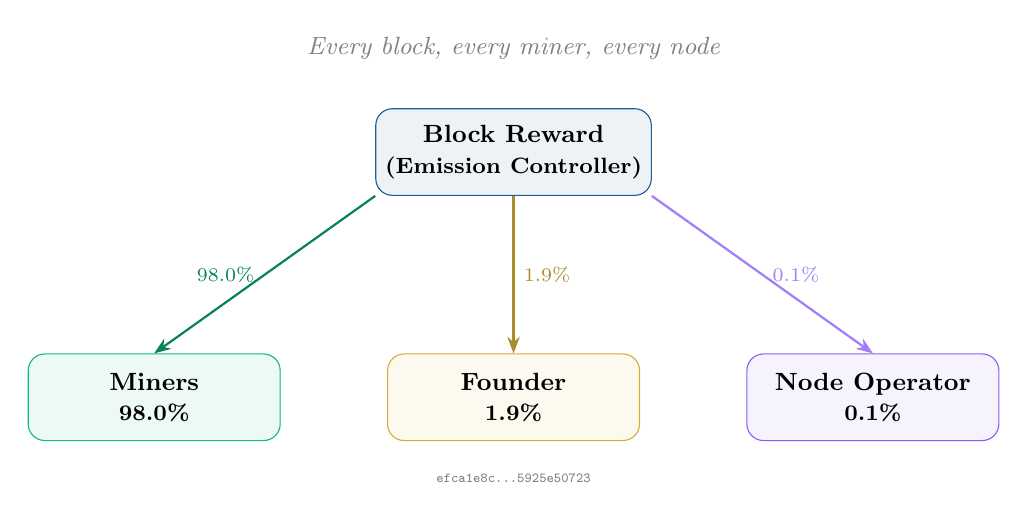
\begin{tikzpicture}[
    node distance=1.8cm,
    box/.style={rectangle, rounded corners=6pt, draw=#1, fill=#1!8,
                minimum width=3.2cm, minimum height=1.1cm, align=center,
                font=\small\bfseries},
    arrow/.style={-{Stealth[length=6pt]}, thick, #1},
]
    % Block reward source
    \node[box=qnkblue] (reward) {Block Reward\\{\footnotesize(Emission Controller)}};

    % Three destinations
    \node[box=quggreen, below left=2.0cm and 1.2cm of reward] (miner)
        {Miners\\{\footnotesize 98.0\%}};
    \node[box=wealthgold, below=2.0cm of reward] (founder)
        {Founder\\{\footnotesize 1.9\%}};
    \node[box=qugpurple, below right=2.0cm and 1.2cm of reward] (operator)
        {Node Operator\\{\footnotesize 0.1\%}};

    % Arrows
    \draw[arrow=quggreen!70!black] (reward.south west) -- (miner.north)
        node[midway, left, font=\scriptsize\color{quggreen!70!black}] {98.0\%};
    \draw[arrow=wealthgold!80!black] (reward.south) -- (founder.north)
        node[midway, right, font=\scriptsize\color{wealthgold!80!black}] {1.9\%};
    \draw[arrow=qugpurple!80] (reward.south east) -- (operator.north)
        node[midway, right, font=\scriptsize\color{qugpurple!80}] {0.1\%};

    % Wallet address
    \node[below=0.3cm of founder, font=\tiny\ttfamily\color{gray}]
        {efca1e8c...5925e50723};

    % Title
    \node[above=0.5cm of reward, font=\small\itshape\color{gray}]
        {Every block, every miner, every node};
\end{tikzpicture}
\caption{Fee flow: block reward distribution across the network.}
\label{fig:fee-flow}
\end{figure}

\begin{principle}[title={\textbf{The Principle}}]
A salary is working income---you stop working, it stops.
A percentage of consensus is net worth---it compounds as long as the
network lives. The difference is not arithmetic; it is architectural.
\end{principle}


% ── Chapter 5 ─────────────────────────────────────────────────────────────────
\section{Rich People Manage Their Money, Poor People Mismanage It}

\epigraph{``Until you show you can handle what you've got, you won't
get any more.''}%
{---T. Harv Eker}

\begin{wealthbox}[title={\raisebox{-0.5pt}{\tiny$\bigstar$} Wealth File \#5}]
``It's not about how much money you make---it's about how much you keep.
And how much you keep depends on how well you manage it.
Rich people manage their money well. Poor people mismanage their
money---or avoid the subject of money altogether.''
\end{wealthbox}

\vspace{0.3cm}

Managing money at the protocol level means managing \emph{precision}.
QUG operates with $10^{24}$ decimal places---24~digits after the decimal
point. A single rounding error, multiplied across millions of blocks,
can create or destroy millions of coins.

In the world of traditional finance, rounding is an accounting
convention. In blockchain, rounding is a consensus-breaking event.

The founder's money management is not a budget spreadsheet. It is
\texttt{u128} arithmetic with \texttt{saturating\_mul}:

\begin{lstlisting}[caption={Precision Money Management (\texttt{emission\_controller.rs})}]
/// Fixed-point precision multiplier for u128 calculations
/// Must satisfy: BASE_ANNUAL_EMISSION * PRECISION < u128::MAX
/// 2.625e30 * 1e6 = 2.625e36 < 3.4e38  (margin: ~130x)
const PRECISION: u128 = 1_000_000;

/// Dynamic per-block safety cap: 2x the ideal reward
pub fn dynamic_max_reward(era: u64, block_rate_bps: f64) -> u128 {
    if era >= 64 { return MIN_REWARD; }
    let target = annual_emission(era);
    let rate = block_rate_bps.clamp(0.001, 100_000.0);
    let expected_blocks = (rate * SECONDS_PER_YEAR) as u128;
    if expected_blocks == 0 { return MIN_REWARD; }
    let ideal = (target * PRECISION) / expected_blocks / PRECISION;
    ideal.saturating_mul(2)
         .clamp(MIN_REWARD, ABSOLUTE_MAX_REWARD_PER_BLOCK)
}
\end{lstlisting}

Every multiplication uses \texttt{saturating\_mul}---if the result would
overflow \texttt{u128} ($3.4 \times 10^{38}$), it clamps to the maximum
instead of wrapping to zero. Every division is checked. Every reward is
bounded between \texttt{MIN\_REWARD} ($10^{19}$, about 0.00001~QUG) and
\texttt{ABSOLUTE\_MAX\_REWARD\_PER\_BLOCK} ($2 \times 10^{24}$, exactly
2.0~QUG).

In the world of finance, wrapping is theft. Clamping is a circuit
breaker.

The coinbase transaction---the transaction that creates new coins---is
marked with a signature that cannot be forged:

\begin{lstlisting}[caption={The Coinbase Marker (\texttt{q-types/src/lib.rs})}]
// Coinbase signature magic marker: [0xC0, 0x1B, 0xA5, 0xE6]
// "COINBASE" encoded in hex + version byte
sig_bytes.extend_from_slice(&[0xC0, 0x1B, 0xA5, 0xE6]);
\end{lstlisting}

\texttt{0xC01BA5E6}---``coinbase'' spelled in hexadecimal, the
programmer's equivalent of a notary seal. Every node verifies this
marker. Every light client can audit it. The money supply is not
a database entry that an administrator can edit; it is a cryptographic
proof that the entire network validates.

\begin{principle}[title={\textbf{The Principle}}]
Managing money means managing precision. When your currency has $10^{24}$
decimal places, a single rounding error is a financial catastrophe.
\texttt{saturating\_mul} is the Rust programmer's budget discipline.
\end{principle}


% ── Chapter 6 ─────────────────────────────────────────────────────────────────
\section{Rich People Have Their Money Work Hard for Them}

\epigraph{``Rich people have their money work hard for them.\\
Poor people work hard for their money.''}%
{---T. Harv Eker}

\begin{wealthbox}[title={\raisebox{-0.5pt}{\tiny$\bigstar$} Wealth File \#6}]
``The most important thing to understand about money is that it is a
tool. Money works for you or you work for money. Rich people see every
dollar as a `seed' that can be planted to earn a hundred more dollars,
which can then be planted to earn a thousand more.''
\end{wealthbox}

\vspace{0.3cm}

While the founder sleeps, block 87{,}342 is produced by a miner in
Berlin. The emission controller computes the reward:
0.0831~QUG. Of that, 1.9\%---0.001579~QUG---flows to
\texttt{efca1e8c...}. The founder did not wake up. Did not check
email. Did not ``hustle.''

Three seconds later, block 87{,}343 is produced by a miner in Seoul.
Another 0.001579~QUG.

Every few seconds, somewhere in the world, a CPU cycles through SHA-256
hashes. The gossipsub protocol propagates the block across four
bootstrap nodes spanning Europe. Tor circuits encrypt the traffic.
Kademlia DHT routes the discovery. Dandelion++ obscures the origin.

And 1.9\% of every reward, from every block, flows to one address.

This is the ultimate expression of Eker's principle: money working for
you. Not a rental property that needs maintenance. Not a stock that
needs monitoring. Not a business that needs employees.
\emph{Consensus itself}---the mathematical heartbeat of a decentralized
network---doing the work.

A rental property has tenants who call at midnight. Consensus has
\texttt{saturating\_mul}, and it never calls.

The node-operator split (0.1\% of the dev fee) incentivizes
decentralization: anyone running a node earns a small share, encouraging
more nodes, which strengthens the network, which produces more blocks,
which generates more fees. A virtuous cycle encoded in seven lines of
Rust:

\begin{lstlisting}[caption={The Virtuous Cycle (\texttt{block\_producer.rs})}]
// v8.6.1: Split dev fee between founder and node operator
let operator_promille = self.node_operator_fee_promille
    .load(std::sync::atomic::Ordering::Relaxed) as u128;
let operator_fee = if operator_promille > 0 {
    dev_fee_amount.saturating_mul(operator_promille) / 1000
} else { 0 };
let founder_fee = dev_fee_amount.saturating_sub(operator_fee);
\end{lstlisting}

\begin{principle}[title={\textbf{The Principle}}]
The ultimate passive income is not dividends or rent---it is a
percentage of consensus. It works while you sleep because it
\emph{is} the network sleeping and waking and producing blocks.
\end{principle}


% ═══════════════════════════════════════════════════════════════════════════════
% PART III: THE NETWORK
% ═══════════════════════════════════════════════════════════════════════════════
\newpage
\begin{center}
{\LARGE\bfseries\color{quggreen!80!black} Part III: The Network}\\[0.3cm]
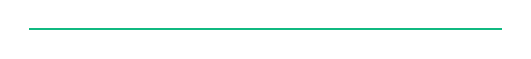
\begin{tikzpicture}
    \draw[quggreen, line width=1pt] (-3,0) -- (3,0);
\end{tikzpicture}
\end{center}
\vspace{0.5cm}

% ── Chapter 7 ─────────────────────────────────────────────────────────────────
\section{Rich People Associate with Positive, Successful People}

\epigraph{``Rich people associate with positive, successful people.\\
Poor people associate with negative or unsuccessful people.''}%
{---T. Harv Eker}

\begin{wealthbox}[title={\raisebox{-0.5pt}{\tiny$\bigstar$} Wealth File \#7}]
``In the real world, your network is your net worth. Energy is contagious.
Either you affect people or you infect people. The same holds true for
the reverse---either people affect you positively or infect you
negatively.''
\end{wealthbox}

\vspace{0.3cm}

A blockchain is, at its core, a network---and Eker's principle applies
literally. Every participant who joins the Q-NarwhalKnight network
makes it stronger: more hash power, more geographic distribution, more
resilience against attacks. Unlike a social circle, however, the
protocol enforces quality mathematically.

By February 2026, the network had grown to:

\begin{itemize}[leftmargin=2em]
    \item \textbf{27+ active miners} submitting solutions across multiple continents
    \item \textbf{4 bootstrap nodes}---Beta (Netherlands), Gamma (Germany),
          Delta (Netherlands), Alpha (testing)---providing network anchor points
    \item \textbf{libp2p gossipsub} for block propagation with cryptographic
          message signing
    \item \textbf{Kademlia DHT} for peer discovery without centralized registries
    \item \textbf{Dandelion++} gossip for privacy-preserving transaction
          broadcast
\end{itemize}

% ── Network Topology Diagram ─────────────────────────────────────────────────
\begin{figure}[H]
\centering
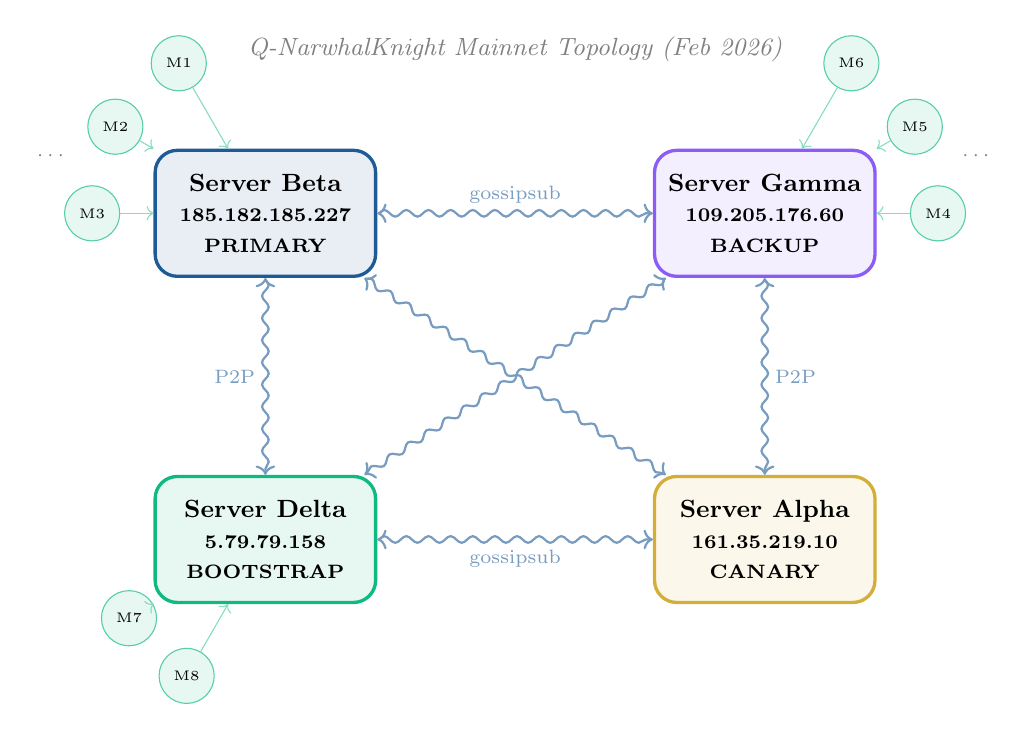
\begin{tikzpicture}[
    node distance=3.5cm,
    server/.style={rectangle, rounded corners=8pt, draw=#1, fill=#1!10,
                   minimum width=2.8cm, minimum height=1.6cm, align=center,
                   font=\small\bfseries, line width=1.2pt},
    miner/.style={circle, draw=quggreen!70, fill=quggreen!10,
                  minimum size=0.7cm, font=\tiny},
    gossip/.style={<->, thick, qnkblue!60, decorate,
                   decoration={snake, amplitude=1.2pt, segment length=8pt}},
]
    % Servers
    \node[server=qnkblue] (beta)  {Server Beta\\{\scriptsize 185.182.185.227}\\{\scriptsize PRIMARY}};
    \node[server=qugpurple, right=3.5cm of beta] (gamma)
        {Server Gamma\\{\scriptsize 109.205.176.60}\\{\scriptsize BACKUP}};
    \node[server=quggreen, below=2.5cm of beta] (delta)
        {Server Delta\\{\scriptsize 5.79.79.158}\\{\scriptsize BOOTSTRAP}};
    \node[server=wealthgold, below=2.5cm of gamma] (alpha)
        {Server Alpha\\{\scriptsize 161.35.219.10}\\{\scriptsize CANARY}};

    % Gossipsub connections
    \draw[gossip] (beta) -- (gamma)
        node[midway, above, font=\scriptsize\color{qnkblue}] {gossipsub};
    \draw[gossip] (beta) -- (delta)
        node[midway, left, font=\scriptsize\color{qnkblue}] {P2P};
    \draw[gossip] (gamma) -- (alpha)
        node[midway, right, font=\scriptsize\color{qnkblue}] {P2P};
    \draw[gossip] (delta) -- (alpha)
        node[midway, below, font=\scriptsize\color{qnkblue}] {gossipsub};
    \draw[gossip] (beta) -- (alpha);
    \draw[gossip] (gamma) -- (delta);

    % Miners around Beta
    \foreach \angle/\label in {120/M1, 150/M2, 180/M3} {
        \node[miner] (m\label) at ($(beta) + (\angle:2.2cm)$) {\label};
        \draw[->, thin, quggreen!50] (m\label) -- (beta);
    }

    % Miners around Gamma
    \foreach \angle/\label in {0/M4, 30/M5, 60/M6} {
        \node[miner] (m\label) at ($(gamma) + (\angle:2.2cm)$) {\label};
        \draw[->, thin, quggreen!50] (m\label) -- (gamma);
    }

    % More miners scattered
    \node[miner] (m7) at ($(delta) + (210:2cm)$) {M7};
    \draw[->, thin, quggreen!50] (m7) -- (delta);
    \node[miner] (m8) at ($(delta) + (240:2cm)$) {M8};
    \draw[->, thin, quggreen!50] (m8) -- (delta);

    % Dots indicating more miners
    \node[font=\scriptsize\color{gray}] at ($(beta) + (165:2.8cm)$) {$\cdots$};
    \node[font=\scriptsize\color{gray}] at ($(gamma) + (15:2.8cm)$) {$\cdots$};

    % Title
    \node[above=1.8cm of $(beta)!0.5!(gamma)$, font=\small\itshape\color{gray}]
        {Q-NarwhalKnight Mainnet Topology (Feb 2026)};
\end{tikzpicture}
\caption{Network topology: 4 bootstrap nodes with 27+ miners connected via gossipsub.}
\label{fig:network-topology}
\end{figure}

The beauty of a decentralized network as ``positive association'' is
that it is \emph{structural}. You cannot have a lazy node---a node
either validates blocks correctly or gets rejected by consensus. There
are no negative participants; the protocol filters them out
mathematically. Eker advises you to choose your friends wisely;
consensus does it for you.

\begin{principle}[title={\textbf{The Principle}}]
In a blockchain, your network literally is your net worth.
Every node that joins makes every other node's coins more valuable.
Consensus is positive association enforced by mathematics.
\end{principle}


% ── Chapter 8 ─────────────────────────────────────────────────────────────────
\section{Rich People Are Willing to Promote Themselves}

\epigraph{``If you believe your product or service can truly fulfill
people, it's your duty to let them know about it.''}%
{---T. Harv Eker}

\begin{wealthbox}[title={\raisebox{-0.5pt}{\tiny$\bigstar$} Wealth File \#8}]
``Resenting promotion is one of the greatest obstacles to success.
People who have issues with selling and promotion are usually broke.
Rich people are willing to promote themselves and their value.''
\end{wealthbox}

\vspace{0.3cm}

Most blockchain founders hide their fee structures in footnotes---or
worse, in token vesting schedules that only a securities lawyer can
parse. The Q-NarwhalKnight founder did the opposite: 71 academic
whitepapers. A public website at \texttt{quillon.xyz}. Open-source
code. A transparent 1.9\% fee that anyone can audit by reading
\texttt{block\_producer.rs} line~1139.

This is not arrogance. It is what Eker calls ``promoting your value.''
The 1.9\% fee is not hidden because hiding it would be a \emph{poverty}
mindset---the belief that earning money from your creation is somehow
shameful.

The promotion includes:

\begin{itemize}[leftmargin=2em]
    \item \textbf{71 academic whitepapers} covering consensus, privacy,
          quantum cryptography, economics, DEX design, AI integration,
          and governance
    \item \textbf{quillon.xyz}---a full-featured web wallet with real-time
          SSE streaming, transaction history, and network statistics
    \item \textbf{A download page} where anyone can get the node binary
          with a single \texttt{wget} command
    \item \textbf{Complete transparency}: every constant, every fee split,
          every wallet address is visible in the source code
\end{itemize}

The 72nd paper is the one you are reading now.

\begin{principle}[title={\textbf{The Principle}}]
Hiding your fee is a poverty mindset. Publishing 72~papers explaining
your architecture, your economics, and your fee structure is the
blockchain equivalent of Eker's self-promotion---shameless, transparent,
and necessary. If you built something worth using, silence is not
humility; it is sabotage.
\end{principle}


% ═══════════════════════════════════════════════════════════════════════════════
% PART IV: THE LAUNCH
% ═══════════════════════════════════════════════════════════════════════════════
\newpage
\begin{center}
{\LARGE\bfseries\color{qugpurple} Part IV: The Launch}\\[0.3cm]
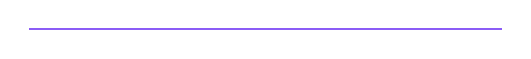
\begin{tikzpicture}
    \draw[qugpurple, line width=1pt] (-3,0) -- (3,0);
\end{tikzpicture}
\end{center}
\vspace{0.5cm}

% ── Chapter 9 ─────────────────────────────────────────────────────────────────
\section{Rich People Act in Spite of Fear}

\epigraph{``Action is the bridge between the inner world and the
outer world.''}%
{---T. Harv Eker}

\begin{wealthbox}[title={\raisebox{-0.5pt}{\tiny$\bigstar$} Wealth File \#9}]
``Comfort is the enemy of achievement. A truly rich person is willing
to act in spite of fear. The key to success is not to try to eliminate
fear---it is to act in spite of it.''
\end{wealthbox}

\vspace{0.3cm}

February 22, 2026. 12:00 UTC. Genesis timestamp \texttt{1771761600}.

The launch procedure reads like a controlled demolition---because it
is one:

\begin{enumerate}[leftmargin=2em]
    \item \textbf{T$-$30\,min}: Stop \emph{all} old servers
          simultaneously. Both must be down before either new one
          starts---this prevents HTTP state-sync contamination from old
          to new.
    \item \textbf{T$-$20\,min}: Update service files with new network ID,
          new database path, new encryption passphrases.
    \item \textbf{T$-$15\,min}: Generate fresh encryption keys from
          \texttt{/dev/urandom}.
    \item \textbf{T$-$10\,min}: Start Beta first (the bootstrap node).
          A new libp2p identity auto-generates.
    \item \textbf{T$-$5\,min}: Start Gamma. Capture its new peer ID.
    \item \textbf{T$\pm$0}: Genesis timestamp reached. Mining begins
          automatically. The first block is produced.
\end{enumerate}

The fear is not irrational. It is specific and technical:

\begin{itemize}[leftmargin=2em]
    \item What if a bug in \texttt{balance\_consensus.rs} creates coins
          from nothing?
    \item What if the emission controller's error correction oscillates
          and mints 34$\times$ the intended supply---\emph{again}?
    \item What if a height regression wipes the chain at block 5{,}000?
    \item What if RocksDB's block cache eats all RAM and OOM-kills the
          bootstrap node during the first hour?
\end{itemize}

Every one of these has happened before. Every one was fixed. But the
fix is in \emph{this} binary, compiled \emph{this} morning, and if
there is a regression that the 4{,}000 tests did not catch---

You act in spite of fear. You type \texttt{systemctl start q-api-server}
and watch the first block appear in the logs:

\begin{lstlisting}[language={}, basicstyle=\ttfamily\footnotesize\color{quggreen!70!black}]
[2026-02-22T12:00:03Z] Block #1 produced: reward=0.0831 QUG
[2026-02-22T12:00:03Z] Coinbase: 98.0% -> miner, 1.9% -> founder
[2026-02-22T12:00:03Z] Network: mainnet2026.2 | Genesis: 1771761600
[2026-02-22T12:00:03Z] P2P: 2 peers connected via gossipsub
\end{lstlisting}

\begin{principle}[title={\textbf{The Principle}}]
Every mainnet launch is an act of faith disguised as engineering.
You cannot eliminate the fear of a consensus bug that destroys everything.
You can only act in spite of it---after writing 4{,}000 tests.
\end{principle}


% ── Chapter 10 ────────────────────────────────────────────────────────────────
\section{Rich People Constantly Learn and Grow}

\epigraph{``Every master was once a disaster.''}%
{---T. Harv Eker}

\begin{wealthbox}[title={\raisebox{-0.5pt}{\tiny$\bigstar$} Wealth File \#10}]
``You can be right or you can be rich, but you can't be both.
Rich people constantly learn and grow. Poor people think they
already know.''
\end{wealthbox}

\vspace{0.3cm}

The version history tells the story of continuous growth:

\begin{table}[H]
\centering
\caption{The Journey from Prototype to Production}
\begin{tabular}{@{}llp{7cm}@{}}
\toprule
\textbf{Version} & \textbf{Date} & \textbf{Lesson} \\
\midrule
v0.2.0-beta  & 2025    & First compilation. Nothing works. \\
v1.4.1-beta  & Late 2025 & Mainnet safety: height-gated validation rules \\
v3.3.7-beta  & Jan 2026  & Connection warmup for new nodes \\
v7.1.5       & Feb 2026  & Configurable dev fee in basis points \\
v7.2.8       & Feb 2026  & Dynamic max reward---fixed 92.5\% under-emission \\
v7.4.1       & Feb 2026  & Height regression fix: \texttt{put\_sync} with \texttt{fsync} \\
v8.0.0       & Feb 2026  & 23-crate comprehensive update \\
v8.5.9       & Feb 2026  & Miner version fix, thread retry, QCredit vault \\
v8.6.4       & Feb 2026  & Current production---emission stable \\
\bottomrule
\end{tabular}
\end{table}

Each version is a lesson Eker would recognize: the version where
floating-point arithmetic was replaced with integer-only computation
(``you can be right or you can be rich''). The version where the
correction-factor smoothing was raised from 0.5 to 0.8 because
wall-clock rate measurement made it safe to be more aggressive
(``constant learning''). The version where
\texttt{cargo clean --package q-api-server} became mandatory after
changing constants, because incremental compilation caches old values
(``every master was once a disaster'').

In traditional software, version numbers are marketing. In blockchain,
they are scar tissue---and scar tissue is stronger than the original
skin.

% ── Emission Halving Curve ────────────────────────────────────────────────────
\begin{figure}[H]
\centering
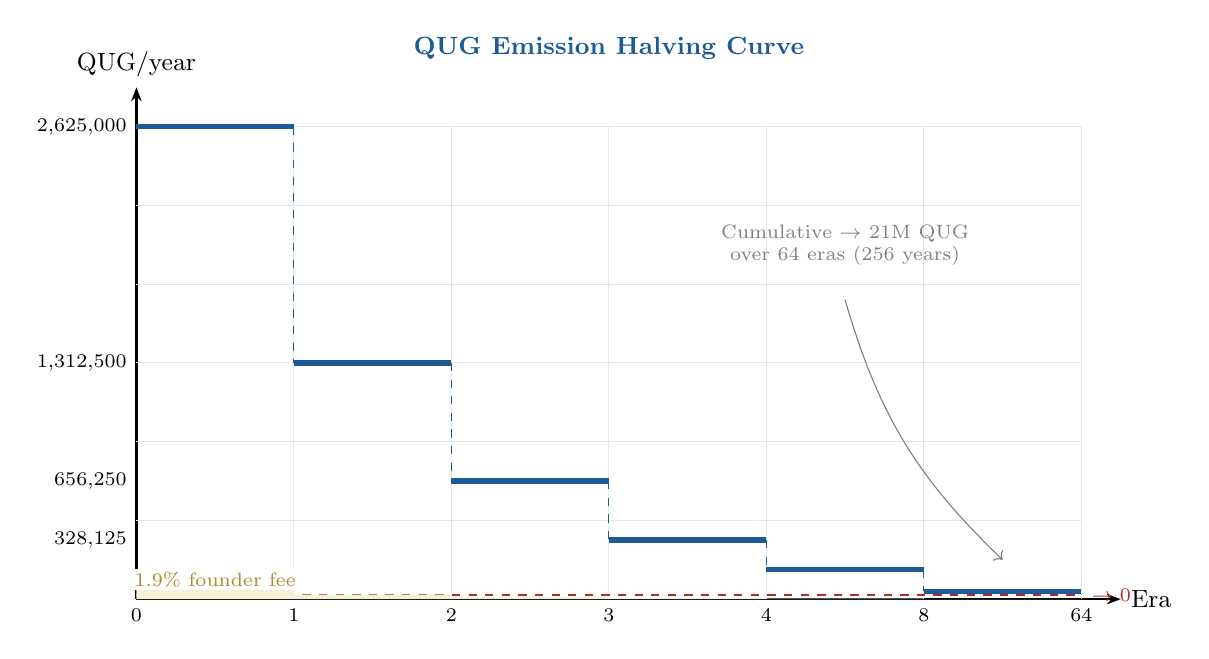
\begin{tikzpicture}[scale=1.0]
    % Axes
    \draw[-{Stealth[length=5pt]}, thick] (0,0) -- (12.5,0)
        node[right, font=\small] {Era};
    \draw[-{Stealth[length=5pt]}, thick] (0,0) -- (0,6.5)
        node[above, font=\small] {QUG/year};

    % Grid lines
    \foreach \y in {1,...,6} {
        \draw[gray!20] (0,\y) -- (12,\y);
    }
    \foreach \x in {2,4,...,12} {
        \draw[gray!20] (\x,0) -- (\x,6);
    }

    % Y-axis labels
    \node[left, font=\scriptsize] at (0,6) {2{,}625{,}000};
    \node[left, font=\scriptsize] at (0,3) {1{,}312{,}500};
    \node[left, font=\scriptsize] at (0,1.5) {656{,}250};
    \node[left, font=\scriptsize] at (0,0.75) {328{,}125};

    % X-axis labels
    \node[below, font=\scriptsize] at (0,0) {0};
    \node[below, font=\scriptsize] at (2,0) {1};
    \node[below, font=\scriptsize] at (4,0) {2};
    \node[below, font=\scriptsize] at (6,0) {3};
    \node[below, font=\scriptsize] at (8,0) {4};
    \node[below, font=\scriptsize] at (10,0) {8};
    \node[below, font=\scriptsize] at (12,0) {64};

    % Halving curve (stepped)
    \draw[qnkblue, line width=2pt]
        (0,6) -- (2,6)
        (2,3) -- (4,3)
        (4,1.5) -- (6,1.5)
        (6,0.75) -- (8,0.75)
        (8,0.375) -- (10,0.375)
        (10,0.1) -- (12,0.1);

    % Dashed drops
    \draw[qnkblue, dashed, thin] (2,6) -- (2,3);
    \draw[qnkblue, dashed, thin] (4,3) -- (4,1.5);
    \draw[qnkblue, dashed, thin] (6,1.5) -- (6,0.75);
    \draw[qnkblue, dashed, thin] (8,0.75) -- (8,0.375);
    \draw[qnkblue, dashed, thin] (10,0.375) -- (10,0.1);

    % 21M asymptote annotation
    \draw[ekerred, dashed, thick] (0,0.05) -- (12,0.05)
        node[right, font=\scriptsize\color{ekerred}] {$\to 0$};

    % 1.9% band (shaded)
    \fill[wealthgold!20]
        (0,0) -- (0,6*0.019) -- (2,6*0.019) -- (2,3*0.019) --
        (4,3*0.019) -- (4,1.5*0.019) -- (6,1.5*0.019) --
        (6,0.75*0.019) -- (8,0.75*0.019) --
        (8,0.375*0.019) -- (10,0.375*0.019) --
        (10,0.1*0.019) -- (12,0.1*0.019) -- (12,0) -- cycle;

    % 1.9% label
    \node[font=\scriptsize\color{wealthgold!80!black}, fill=white, inner sep=1pt]
        at (1,0.25) {1.9\% founder fee};

    % Cumulative supply annotation
    \node[font=\scriptsize\color{gray}, align=center] at (9,4.5)
        {Cumulative $\to$ 21M QUG\\over 64 eras (256 years)};
    \draw[->, thin, gray] (9,3.8) to[bend right=15] (11,0.5);

    % Title
    \node[font=\small\bfseries\color{qnkblue}, align=center] at (6,7)
        {QUG Emission Halving Curve};
\end{tikzpicture}
\caption{Emission schedule: annual emission halves every 4 years for 64 eras,
asymptotically approaching the 21M QUG supply cap. The gold band represents
the 1.9\% founder fee.}
\label{fig:emission-curve}
\end{figure}

The 4{,}000-test suite is perhaps the purest expression of ``constant
learning'': every bug that was found became a test that ensures it can
never happen again. The tests are not bureaucracy---they are
\emph{institutional memory}, a system that learns from its own mistakes
and compiles the lessons into guarantees.

\begin{principle}[title={\textbf{The Principle}}]
Version numbers are a growth journal. Each increment represents a bug
found, a lesson learned, a system made more resilient. The founder who
stops learning stops growing---and in blockchain, that means the
network dies.
\end{principle}


% ═══════════════════════════════════════════════════════════════════════════════
% PART V: THE LONG VIEW
% ═══════════════════════════════════════════════════════════════════════════════
\newpage
\begin{center}
{\LARGE\bfseries\color{ekerred!80!black} Part V: The Long View}\\[0.3cm]
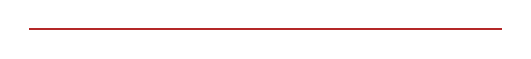
\begin{tikzpicture}
    \draw[ekerred, line width=1pt] (-3,0) -- (3,0);
\end{tikzpicture}
\end{center}
\vspace{0.5cm}

% ── Chapter 11 ────────────────────────────────────────────────────────────────
\section{After the Last Coin: The Post-Emission Economy}

\epigraph{``The goal of creating wealth is not to just have money.\\
The goal is freedom.''}%
{---T. Harv Eker}

\begin{wealthbox}[title={\raisebox{-0.5pt}{\tiny$\bigstar$} Wealth File \#11}]
``Rich people think long term. They balance their spending on enjoyment
today with investing for freedom tomorrow. Poor people think short
term. They run their lives based on immediate gratification.''
\end{wealthbox}

\vspace{0.3cm}

Every emission schedule has an endpoint. Bitcoin's last satoshi will be
mined around the year 2140. QUG's last fractional coin will be emitted
around the year 2282. What happens to the 1.9\% founder fee when there
are no more block rewards to take 1.9\% of?

The answer is built into the design: transaction fees.

As emission decreases across 64~halving eras, the network transitions
from an emission-funded model to a fee-funded model---the same
transition Bitcoin faces, but with 256~years of runway instead of 120.
During this transition:

\begin{itemize}[leftmargin=2em]
    \item \textbf{Early eras (0--8)}: Block rewards dominate. The 1.9\%
          fee provides steady founder income from emission.
    \item \textbf{Middle eras (8--32)}: Emission shrinks. If the network
          has achieved adoption, transaction fees grow to compensate.
          The DEX, smart contracts, and stablecoin system all generate
          on-chain activity---and fees.
    \item \textbf{Late eras (32--64)}: Emission is negligible.
          Transaction fees sustain miners and, through them, the founder
          fee. The network is self-sustaining or it is not---there is
          no central bank to print more.
\end{itemize}

This is the honest answer: the 1.9\% fee's long-term value depends
entirely on whether the network achieves real adoption. It is not a
guaranteed income stream; it is an \emph{incentive-aligned bet} that the
founder's continued work will make the network valuable enough to
generate transaction volume.

Eker would approve: the founder's wealth is tied directly to the
network's success. There is no golden parachute. No vesting cliff
after which the founder can walk away. The incentive alignment is
permanent and immutable---encoded in consensus, not in a contract that
a lawyer can renegotiate.

\begin{principle}[title={\textbf{The Principle}}]
A truly long-term financial blueprint accounts for its own expiration.
The 1.9\% fee is not forever---it lasts exactly as long as emission
does. After that, value must come from utility, not from minting.
That constraint is a feature, not a bug.
\end{principle}


% ── Chapter 12 ────────────────────────────────────────────────────────────────
\section{Governance: Who Controls the Thermostat?}

\epigraph{``If you want to change the fruits, you will first have to
change the roots.''}%
{---T. Harv Eker}

A natural question arises: if the 1.9\% fee is hardcoded into consensus,
who can change it? What if the community decides the fee should be
1.0\%, or 0\%, or 3\%?

The current answer is direct: the fee is a constant in
\texttt{block\_producer.rs}. Changing it requires a code change, a new
binary, and every node operator choosing to upgrade. This is
governance by rough consensus---the same model Bitcoin uses for its
block size, its halving schedule, and its scripting language.

No DAO vote can override it. No token-weighted governance can force it.
The fee changes only if the people running the nodes choose to run a
binary that changes it. This is slower than on-chain governance, more
conservative than a multisig---and, the founder would argue, more
resistant to capture.

The \texttt{dev\_fee\_bps} variable is an \texttt{AtomicU64}, which means
it \emph{can} be adjusted at runtime via configuration. But the default
is 190~basis points, and changing it requires deliberate, transparent
action by the node operator. No silent extraction. No backdoor.

\begin{principle}[title={\textbf{The Principle}}]
The best governance is the kind where changing the rules requires
convincing every participant to update their software. It is slow,
it is conservative, and it is the most censorship-resistant form of
governance ever invented.
\end{principle}


% ═══════════════════════════════════════════════════════════════════════════════
% EPILOGUE
% ═══════════════════════════════════════════════════════════════════════════════
\newpage
\begin{center}
{\LARGE\bfseries\color{wealthgold!80!black} Epilogue}\\[0.2cm]
{\Large\color{qnkblue}\itshape The Quantum Millionaire's Creed}\\[0.3cm]

\begin{tikzpicture}
    \draw[wealthgold, line width=2pt] (-4,0) -- (4,0);
    \node[wealthgold, font=\Large] at (0,0.4) {$\bigstar$};
\end{tikzpicture}
\end{center}
\vspace{0.5cm}

T.~Harv Eker ends \emph{Secrets of the Millionaire Mind} with
declarations---statements you speak aloud to reprogram your financial
blueprint. Here are ten declarations for the blockchain builder.

\begin{declaration}[title={\textbf{The Quantum Millionaire's Ten Declarations}}]

\begin{enumerate}[leftmargin=2em, itemsep=0.6em]

\item \textbf{``My code is my financial blueprint.''}\\
I do not inherit a money story from society. I write my own---in Rust,
with \texttt{u128} precision, compiled to machine code, verified by
4{,}000 tests.

\item \textbf{``I think big: 80~crates, 256~years, 21~million coins.''}\\
I do not fork someone else's vision. I build from first principles,
even when the world says it is too ambitious, too complex, too early
for quantum threats that do not yet exist.

\item \textbf{``I am committed, not merely interested.''}\\
I fix the 34$\times$ emission bug at 3~AM. I diagnose the 26.9~GB
memory leak. I count zeros in 31-digit constants. Interest takes
weekends off. Commitment does not.

\item \textbf{``I focus on net worth, not working income.''}\\
I earn a percentage of every block reward---not a salary that stops
when I stop. Consensus works while I sleep. My income is a function
of the network's hash rate, not my hours.

\item \textbf{``I manage my money with \texttt{saturating\_mul}.''}\\
I use $10^{24}$ decimal precision. I clamp every calculation between
\texttt{MIN\_REWARD} and \texttt{ABSOLUTE\_MAX\_REWARD}. I mark every
coinbase with \texttt{0xC01BA5E6}. Overflow is not a rounding error---it
is a financial catastrophe I refuse to allow.

\item \textbf{``I have my money work hard for me.''}\\
Every miner on every continent sends a fraction to
\texttt{efca1e8c...} with every block. I did not ask them to. Consensus
asked them to. The code asked them to. The math asked them to.

\item \textbf{``My network is my net worth.''}\\
27 miners. 4 bootstrap nodes. Gossipsub, Kademlia, Dandelion++. Every
node that joins makes every coin more valuable. I do not compete with my
network---I \emph{am} my network.

\item \textbf{``I promote my value transparently.''}\\
72~whitepapers. Open source. A public fee structure anyone can audit at
\texttt{block\_producer.rs} line~1139. I do not hide my fee because
hiding income is a poverty mindset.

\item \textbf{``I act in spite of fear.''}\\
I type \texttt{systemctl start q-api-server} on mainnet launch day
knowing that a single bug in \texttt{balance\_consensus.rs} could destroy
everything. I act anyway---after writing 4{,}000 tests.

\item \textbf{``I constantly learn and grow.''}\\
v0.2.0-beta to v8.6.4. Hundreds of versions. Each bug a lesson, each
lesson a test, each test a guarantee that the mistake can never recur.
I do not fear mistakes---I compile them into wisdom.

\end{enumerate}
\end{declaration}

\vspace{1cm}

\begin{center}

\begin{tikzpicture}
    \draw[wealthgold, line width=1pt] (-5,0) -- (5,0);
\end{tikzpicture}
\end{center}

\vspace{0.3cm}

\begin{center}
\large\itshape\color{qnkblue}
``The blockchain does not care about your feelings.\\
It cares about your constants.\\[0.3cm]
And your constants had better be right---\\
because 27~miners are counting on them.''\\[0.5cm]
\normalsize\upshape\color{gray}
---The Q-NarwhalKnight Founder
\end{center}

\vspace{1cm}

\begin{center}

\begin{tikzpicture}
    \draw[wealthgold, line width=2pt] (-5,0) -- (5,0);
    \node[wealthgold, font=\Large] at (0,0.4) {$\bigstar$};
\end{tikzpicture}
\end{center}

\vspace{1cm}

% ── Colophon ──────────────────────────────────────────────────────────────────
\begin{center}
\small\color{gray}
\textbf{Q-NarwhalKnight} --- Quantum-Enhanced DAG-BFT Consensus\\
\url{https://quillon.xyz}\\[0.3cm]
\textit{Inspired by T. Harv Eker's ``Secrets of the Millionaire Mind''}\\
\textit{and the real journey of building a blockchain from zero to mainnet.}\\[0.3cm]
February 2026 \quad$\cdot$\quad Version 1.1 \quad$\cdot$\quad Paper \#72
\end{center}

\end{document}
